\usepackage{tkz-graph}
\usepackage{mathtools}
\usepackage{xcolor}
\usepackage{afterpage}
\usepackage{pifont,mdframed}
\usepackage[bottom]{footmisc}

\makeatletter
\gdef\this@inputfilename{input.txt}
\gdef\this@outputfilename{output.txt}
\makeatother

\newcommand{\inputfile}{\texttt{input.txt}}
\newcommand{\outputfile}{\texttt{output.txt}}

\newenvironment{warning}
  {\par\begin{mdframed}[linewidth=2pt,linecolor=gray]%
    \begin{list}{}{\leftmargin=1cm
                   \labelwidth=\leftmargin}\item[\Large\ding{43}]}
  {\end{list}\end{mdframed}\par}
  
Installare una rete affidabile che serva centinaia o migliaia di computer non è un compito facile. Gabriele, incaricato della rete per le prossime nazionali, lo sa bene, e di certo non vuole fare brutta figura proprio davanti gli occhi della commissione olimpica delle Olimpiadi di Informatica. Generalmente la topologia di una rete rientra in una di queste 3 categorie, per ognuna delle quali viene fornito un esempio:

\begin{table}[htbp]
\usetikzlibrary{fit}
\newcommand\addvmargin[1]{
  \node[fit=(current bounding box),inner ysep=#1,inner xsep=0]{};
}
\begin{tabular}{|c|>{\centering\let\newline\\\arraybackslash\hspace{0pt}}m{13.3cm}|}
\hline
Topologia lineare & 

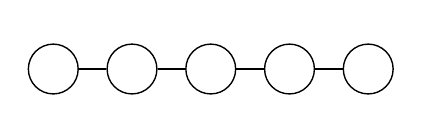
\begin{tikzpicture}[baseline=0]
\GraphInit[vstyle=Normal]
\SetVertexNoLabel
\SetGraphUnit{1}
\Vertices{line}{1,2,3,4,5}
\Edges(1,2,3,4,5)
\addvmargin{2mm}
\end{tikzpicture}
\\
\hline
Topologia ad anello & 

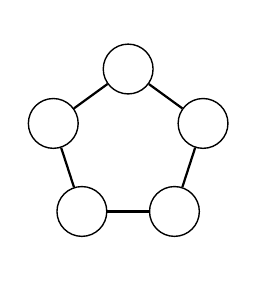
\begin{tikzpicture}[baseline=0, rotate = 90]
\GraphInit[vstyle=Normal]
\SetVertexNoLabel
\SetGraphUnit{1}
\Vertices{circle}{1,2,3,4,5}
\Edges(1,2,3,4,5,1)
\addvmargin{2mm}
\end{tikzpicture}
\\
\hline
Topologia a stella & 
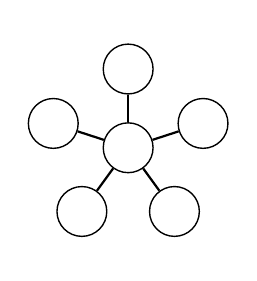
\begin{tikzpicture}[baseline=0, rotate = 90]
\GraphInit[vstyle=Normal]
\SetVertexNoLabel
\SetGraphUnit{1}
\Vertex{0};
\Vertices{circle}{1,2,3,4,5}
\Edges(1,0,2);
\Edges(3,0,4);
\Edges(0,5);
\addvmargin{2mm}
\end{tikzpicture}
\\
\hline
\end{tabular}
\end{table}

Affinché si possa dire che un gruppo connesso di PC formi una certa topologia è necessario che siano presenti almeno due PC nel gruppo. Inoltre le topologie ad anello e a stella necessitano, rispettivamente, di almeno 3 ed almeno 4 PC. I computer lasciati scollegati non formano alcuna topologia di rete.

Gabriele ha già cominciato a collegare i PC con dei cavi, così che certi gruppi di computer sono connessi tra di loro secondo una qualche topologia. Purtroppo non è sempre stato coerente e non ricorda come ha collegato certi pc. Aiuta Gabriele a scrivere un programma che, analizzando la struttura della rete, determina quanti gruppi (connessi) di computer sono collegati rispettando la topologia lineare, quanti quella ad anello e quanti quella a stella.

\InputFile
Il file \inputfile{} è composto da $M+1$ righe. La prima riga contiene gli interi $N$ e $M$, rispettivamente il numero di PC e di cavi presenti nel grafo della rete. Seguono $M$ righe: ognuna contiene due interi $A$ e $B$ separati da uno spazio e rappresenta un cavo (bidirezionale) che collega il PC $A$ con il PC $B$. Gli $N$ PC sono numerati a partire da 1.

\OutputFile
Il file \outputfile{} è composto da una sola riga contenente tre numeri interi separati da spazio: il numero di topologie lineari, ad anello e a stella presenti nella rete.

\pagebreak
\Implementation
Dovrai sottoporre esattamente un file con estensione \texttt{.c}, \texttt{.cpp} o \texttt{.pas}.

\begin{warning}
Tra gli allegati a questo task troverai un template (\texttt{topologia.c}, \texttt{topologia.cpp}, \texttt{topologia.pas}) con un esempio di implementazione da completare.
\end{warning}

Se sceglierai di utilizzare il template, dovrai implementare la seguente funzione:
\begin{center}\begin{tabularx}{\textwidth}{|c|X|}
\hline
C/C++  & \verb|void analizza(int N, int M, int *A, int *B, int *T);|\\
\hline
Pascal & \verb|procedure analizza(N, M: longint; var A, B, T: array of longint);|\\
\hline
\end{tabularx}\end{center}
In cui:
\begin{itemize}[nolistsep]
  \item L'intero $N$ rappresenta il numero di PC.
  \item L'intero $M$ rappresenta il numero di collegamenti nella rete.
  \item Gli array \texttt{A} e \texttt{B} sono indicizzati da $0$ a $M-1$, e rappresentano i collegamenti della rete: per ogni $i=0,\dots, M-1$, vi è un cavo che collega il PC \texttt{A[i]} e il PC \texttt{B[i]}. I PC sono numerati da $1$ a $N$. I collegamenti sono bidirezionali.
  \item La funzione dovrà riempire l'array \texttt{T} con i seguenti tre valori: il numero di topologie lineari, ad anello e a stella, rispettivamente.
\end{itemize}
Il contenuto dell'array \texttt{T} verrà stampato sul file di output.

% Assunzioni
\Constraints
\begin{itemize}[nolistsep, itemsep=2mm]
  \item $2 \le N \le 100\,000$.
  \item $1 \le M \le 100\,000$.
  \item Un cavo non collega mai un PC con se stesso.
  \item Non esistono due cavi distinti che collegano la stessa coppia di PC.
\end{itemize}

\Scoring
Il tuo programma verrà testato su diversi test case raggruppati in subtask.
Per ottenere il punteggio relativo ad un subtask, è necessario risolvere
correttamente tutti i test relativi ad esso.

\begin{itemize}[nolistsep,itemsep=2mm]
  \item \textbf{\makebox[2cm][l]{Subtask 1} [10 punti]}: Casi d'esempio.
  \item \textbf{\makebox[2cm][l]{Subtask 2} [20 punti]}: $N \leq 10$.
  \item \textbf{\makebox[2cm][l]{Subtask 3} [40 punti]}: La rete dei PC è connessa.
  \item \textbf{\makebox[2cm][l]{Subtask 4} [30 punti]}: Nessuna limitazione specifica.
\end{itemize}

% Esempi
\Examples
\begin{example}
\exmp{
15 11
2 8
3 14
12 2
9 11
12 8
4 14
7 1
6 5
10 1
14 13
1 6
}{%
1 1 1
}%
\end{example}

\Explanation
Nel caso di esempio la rete è la seguente:\\[1cm]
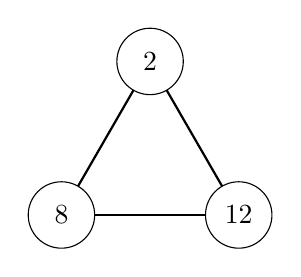
\begin{tikzpicture}[baseline = 0,rotate = 90]
\GraphInit[vstyle=Normal]

\tikzset{VertexStyle/.style = {%
shape = circle,
minimum size = 24pt,draw}}

\SetGraphUnit{1.3}
\Vertices{circle}{2,8,12}
\Edges(2,8,12,2)
\end{tikzpicture}
\hfill
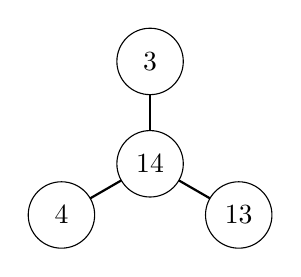
\begin{tikzpicture}[baseline = 0, rotate=90]
\GraphInit[vstyle=Normal]

\tikzset{VertexStyle/.style = {%
shape = circle,
minimum size = 24pt,draw}}

\SetGraphUnit{1.3}
\Vertex{14}
\Vertices{circle}{3,4,13}
\Edges(3,14,13)
\Edges(14,4)
\end{tikzpicture}
\hfill
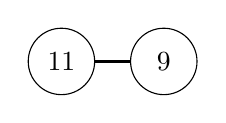
\begin{tikzpicture}[baseline = 0]
\GraphInit[vstyle=Normal]

\tikzset{VertexStyle/.style = {%
shape = circle,
minimum size = 24pt,draw}}

\SetGraphUnit{1.3}
\Vertices{line}{11,9}
\Edges(11,9)
\end{tikzpicture}
\hfill
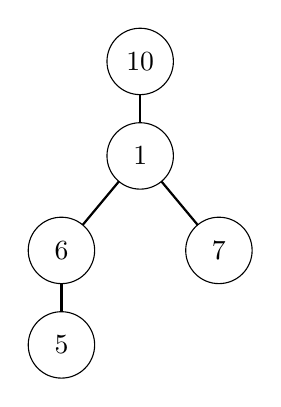
\begin{tikzpicture}[baseline = 0, y=1.2cm]
\GraphInit[vstyle=Normal]

\tikzset{VertexStyle/.style = {%
shape = circle,
minimum size = 24pt,draw}}

\Vertex{1}
\NO(1){10}
\SOWE(1){6}
\SO(6){5}
\SOEA(1){7}
\Edges(10,1,6,5)
\Edges(1,7)
\end{tikzpicture}
\hfill
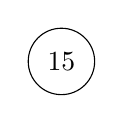
\begin{tikzpicture}[baseline = 0]
\GraphInit[vstyle=Normal]

\tikzset{VertexStyle/.style = {%
shape = circle,
minimum size = 24pt,draw}}

\Vertex{15}
\end{tikzpicture}
\\[.1cm]

Osserviamo che la rete non è connessa. La prima \emph{componente connessa} corrisponde ad una topologia ad anello (ovvero, la sottorete composta dai nodi $2$, $8$ e $12$), la seconda invece corrisponde ad una topologia a stella (nella quale il nodo $14$ rappresenta il centro) e la terza ad una topologia lineare (nodi $11$ e $9$). La quarta e la quinta componente connessa non corrispondono a nessuna delle topologie descritte nel testo.

\end{document}
